\documentclass{beamer}
\mode<presentation>
\usepackage{amsmath}
\usepackage{amssymb}
%\usepackage{advdate}
\usepackage{graphicx}
\usepackage{adjustbox}
\usepackage{subcaption}
\usepackage{enumitem}
\usepackage{multicol}
\usepackage{mathtools}
\usepackage{listings}
\usepackage{url}
\def\UrlBreaks{\do\/\do-}
\usetheme{Boadilla}
\usecolortheme{lily}
\setbeamertemplate{footline}
{
  \leavevmode%
  \hbox{%
  \begin{beamercolorbox}[wd=\paperwidth,ht=2.25ex,dp=1ex,right]{author in head/foot}%
    \insertframenumber{} / \inserttotalframenumber\hspace*{2ex} 
  \end{beamercolorbox}}%
  \vskip0pt%
}
\setbeamertemplate{navigation symbols}{}

\providecommand{\nCr}[2]{\,^{#1}C_{#2}} % nCr
\providecommand{\nPr}[2]{\,^{#1}P_{#2}} % nPr
\providecommand{\mbf}{\mathbf}
\providecommand{\pr}[1]{\ensuremath{\Pr\left(#1\right)}}
\providecommand{\qfunc}[1]{\ensuremath{Q\left(#1\right)}}
\providecommand{\sbrak}[1]{\ensuremath{{}\left[#1\right]}}
\providecommand{\lsbrak}[1]{\ensuremath{{}\left[#1\right.}}
\providecommand{\rsbrak}[1]{\ensuremath{{}\left.#1\right]}}
\providecommand{\brak}[1]{\ensuremath{\left(#1\right)}}
\providecommand{\lbrak}[1]{\ensuremath{\left(#1\right.}}
\providecommand{\rbrak}[1]{\ensuremath{\left.#1\right)}}
\providecommand{\cbrak}[1]{\ensuremath{\left\{#1\right\}}}
\providecommand{\lcbrak}[1]{\ensuremath{\left\{#1\right.}}
\providecommand{\rcbrak}[1]{\ensuremath{\left.#1\right\}}}
\theoremstyle{remark}
\newtheorem{rem}{Remark}
\newcommand{\sgn}{\mathop{\mathrm{sgn}}}
\providecommand{\abs}[1]{$\left\vert#1\right\vert$}
\providecommand{\res}[1]{\Res\displaylimits_{#1}} 
\providecommand{\norm}[1]{\lVert#1\rVert}
\providecommand{\mtx}[1]{\mathbf{#1}}
\providecommand{\mean}[1]{E$\left[ #1 \right]$}
\providecommand{\fourier}{\overset{\mathcal{F}}{ \rightleftharpoons}}
%\providecommand{\hilbert}{\overset{\mathcal{H}}{ \rightleftharpoons}}
\providecommand{\system}[1]{\overset{\mathcal{#1}}{ \longleftrightarrow}}
%\providecommand{\system}{\overset{\mathcal{H}}{ \longleftrightarrow}}
	%\newcommand{\solution}[2]{\textbf{Solution:}{#1}}
%\newcommand{\solution}{\noindent \textbf{Solution: }}
\providecommand{\dec}[2]{\ensuremath{\overset{#1}{\underset{#2}{\gtrless}}}}
\newcommand{\myvec}[1]{\ensuremath{\begin{pmatrix}#1\end{pmatrix}}}
\let\vec\mathbf

\lstset{
%language=C,
frame=single, 
breaklines=true,
columns=fullflexible
}

\numberwithin{equation}{section}

\title{2.6.35}
\author{AI25BTECH11024 - Pratyush Panda}
\begin{document}
\maketitle

\begin{frame}
\textbf{Question: } \\
The value of $\hat{\Vec{i}}.\brak{\hat{\Vec{j}} \times \hat{\Vec{k}}} + \hat{\Vec{j}}.\brak{\hat{\Vec{i}} \times \hat{\Vec{k}}} + \hat{\Vec{k}}.\brak{\hat{\Vec{i}} \times \hat{\Vec{j}}}$ is \underline{\hspace{2cm}}
\end{frame}

\begin{frame}
\textbf{Solution: } \\
Given:
\begin{align}
\Vec{\hat{i}}=\Vec{e_1}=\myvec{1 \\ 0 \\ 0}, \, \Vec{\hat{j}}=\Vec{e_2}=\myvec{0 \\ 1 \\ 0}, \, \Vec{\hat{k}}=\Vec{e_3}=\myvec{0 \\ 0 \\ 1}
\end{align}

Each term of the expression in the question can be found using the scalar triple product determinant.\\
The first term can be written as:
\begin{align}
\brak{\hat{\Vec{i}}.\brak{\hat{\Vec{j}} \times \hat{\Vec{k}}}} = 
\myvec{e_1 && e_2 && e_3} =
\myvec{1 && 0 && 0 \\
       0 && 1 && 0 \\
       0 && 0 && 1}
\end{align}
Determinant of this matrix is 1. Thus, the value of first term is 1.
\end{frame}

\begin{frame}
The second term can be written as:
\begin{align}
\brak{\hat{\Vec{j}}.\brak{\hat{\Vec{i}} \times \hat{\Vec{k}}}} = 
\myvec{e_2 && e_3 && e_1} =
\myvec{0 && 0 && 1 \\
       1 && 0 && 0 \\
       0 && 1 && 0}
\end{align}
Determinant of this matrix is -1. Thus, the value of first term is -1.

The third term can be written as:
\begin{align}
\brak{\hat{\Vec{k}}.\brak{\hat{\Vec{i}} \times \hat{\Vec{j}}}} = 
\myvec{e_3 && e_1 && e_2} =
\myvec{0 && 1 && 0 \\
       0 && 0 && 1 \\
       1 && 0 && 0}
\end{align}
Determinant of this matrix is 1. Thus, the value of first term is 1.
\end{frame}

\begin{frame}
So, the sum of all the terms is;
\begin{align}
\hat{\Vec{i}}.\brak{\hat{\Vec{j}} \times \hat{\Vec{k}}} + \hat{\Vec{j}}.\brak{\hat{\Vec{i}} \times \hat{\Vec{k}}} + \hat{\Vec{k}}.\brak{\hat{\Vec{i}} \times \hat{\Vec{j}}} = 1 + (-1) + 1
\end{align}
\begin{align}
or, \, \hat{\Vec{i}}.\brak{\hat{\Vec{j}} \times \hat{\Vec{k}}} + \hat{\Vec{j}}.\brak{\hat{\Vec{i}} \times \hat{\Vec{k}}} + \hat{\Vec{k}}.\brak{\hat{\Vec{i}} \times \hat{\Vec{j}}} = 1
\end{align}
\end{frame}

\begin{frame}
\begin{figure}[H]
\centering
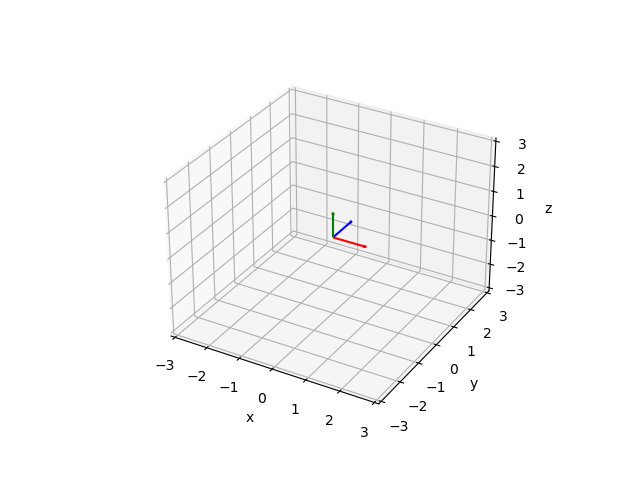
\includegraphics[width=0.6\columnwidth]{figs/img.png}
\caption*{}
\end{figure}
\end{frame}

\end{document}
